\documentclass[	DIV=calc,
							paper=a4,
							fontsize=12pt,
							onecolumn]{scrartcl}	 				

\usepackage{lipsum}												
\usepackage[brazil]{babel}										
\usepackage[protrusion=true,expansion=true]{microtype}				
\usepackage{amsmath,amsfonts,amsthm}					
\usepackage[pdftex]{graphicx}								
\usepackage[svgnames]{xcolor}									
\usepackage[hang, small,labelfont=bf,up,textfont=it,up]{caption}	
\usepackage{epstopdf}											
\usepackage{subfig}												
\usepackage{booktabs}											
\usepackage{fix-cm}													
\usepackage[utf8]{inputenc}
\usepackage[top=2.5cm, bottom=2.5cm, left=2.5cm, right=2.5cm]{geometry}
\usepackage[ddmmyyyy]{datetime}
\addto\captionsenglish{%
	\renewcommand\tablename{Tabela}
	\renewcommand\figurename{Figura}
} 
 
\usepackage{sectsty}												
\allsectionsfont{%														
	\usefont{OT1}{phv}{b}{n}									
	}

\sectionfont{%															
	\usefont{OT1}{phv}{b}{n}									
	}

\usepackage{fancyhdr}												
	\pagestyle{fancy}														
\usepackage{lastpage}	

\lhead{}
\chead{}
\rhead{}

\lfoot{\footnotesize \texttt{Cabeamento estruturado} \textbullet ~Modelo de projeto}


\cfoot{}
\rfoot{\footnotesize página \thepage\ de \pageref{LastPage}}
\renewcommand{\headrulewidth}{0.0pt}
\renewcommand{\footrulewidth}{0.4pt}

\usepackage{lettrine}
\newcommand{\initial}[1]{%
     \lettrine[lines=3,lhang=0.3,nindent=0em]{
     				\color{DarkGoldenrod}
     				{\textsf{#1}}}{}}

\usepackage{titling}

\newcommand{\HorRule}{\color{DarkGoldenrod}
									  	\rule{\linewidth}{1pt}%
										}

\pretitle{\vspace{-30pt} \begin{flushleft} \HorRule 
				\fontsize{50}{50} \usefont{OT1}{phv}{b}{n} \color{DarkRed} \selectfont 
				}

\title{Projeto de Cabeamento Estruturado para o Bloco E7 da UTFPR - Campus Santa Helena}					

\posttitle{\par\end{flushleft}\vskip 0.5em}

\preauthor{\begin{flushleft}
					\large \lineskip 0.5em \usefont{OT1}{phv}{b}{sl} \color{DarkRed}}
\author{Joéslei Brunetto}  


\postauthor{\footnotesize \usefont{OT1}{phv}{m}{sl} \color{Black} 
					\\Universidade Tecnológica Federal do Paraná - Câmpus Cornélio Procópio 							
					\par\end{flushleft}\HorRule}

\date{}	

\begin{document}
\maketitle
\thispagestyle{fancy} 	
\thispagestyle{empty}	 

\initial{R}\textbf{eestruturar bloco da UTFPR - Campus Santa Helena, criando uma estrutura de cabeamento para ambientes que no momento dispõe apenas de internet wireless. Serão abordados equipamentos com hacks, switchs, patch panels, voice painels, cabeamentos e pontos de conectividade. Este projeto abrangerá levantamento da planta física, elaboração da planta lógica, equipamentos passivos da rede, levantamento de quantidade/custo e plano de certificação e orçamento.}

%% ====================================
\begin{figure}
	\centering
	
\includegraphics{utfpr}
\end{figure}

\vspace{2cm}
\centerline{\textit{\textbf{\today}}}

\clearpage
    \renewcommand*\listfigurename{Lista de figuras}
\listoffigures

\renewcommand*\listtablename{Lista de tabelas}
\listoftables

\clearpage
\renewcommand{\contentsname}{Sumário}
\tableofcontents
\clearpage

\section{Introdução}
Projeto de rede cabeada para os espaços denominados como salas de professores. Sala esta dos professores do curso de Ciência da Computação. A sala será subdividida em baias totalizando 16 (dezesseis) espaços, alocando-se dois professores por baia. Além dos 32 (trinta e dois) pontos de entrada de rede para os professores, necessita-se também de 32 pontos extras para futura instalação de telefonia voip, sendo dois por baia, ou um por baia sobrando um ponto para qualquer outra utilização. Por fim um ponto para uma impressora de uso comunitário.
Será adicionada ao espaço uma rack de 12U de fixação aérea, com os respectivos equipamentos necessários para a estrutura de lógica como switchs e patch panels. A conexão virá de infraestrutura de rede cabeada já existente, sendo necessário somente a passagem cabeada partindo do switch mais próximo ao local.

 
\subsection{Benefícios}
Esperamos com este projeto melhorar a disponibilidade de internet nos ambientes e ampliação da gerencia sobre os equipamentos na conexão cabeada.

\subsection{Organizações Envolvidas}
O projeto físico será executado pela Diretoria de Planejamento do campus com a atualização da planta baixa.
O projeto de lógica será desenvolvido pela Coordenadoria de Gestão de Tecnologia de Informação.
A execução do projeto será divido entre o Departamento de Serviços Gerais e a Coordenadoria de Gestão de Tecnologia de Informação.

\section{Estado atual}
Atualmente a sala citada dispõe apenas de conexão wireless providas de um access point fixado no teto de um corredor próximo.

\section{Requisitos}
Os requisitos do projeto são:
- Fixação da rack.
- Instalação das eletrocalhas para passagem da lógica nos pontos determinados no projeto.
- Passagem do cabeamento de lógica, inclusive o cabo provindo da estrutura de rede já existente.
- Configuração e instalação de switchs e patch panels na rack.
- Crimpagem dos cabos tanto na extremidade dos patch panels como nos conectores RJ-45 fêmea nos pontos de acesso.
- Certificação dos pontos de lógica.
- Conectorização entre os switchs e patch panels.
- Cabeamento dos equipamentos.
- Configurações dos equipamentos.

\section{Usuários e Aplicativos}

O perfil de usuário limita-se a professores de informática somente, pois estes espaços são exclusivos para os mesmos. 

\subsection{Usuários}

Relação da quantidade x perfil de usuários:
Máximo 16 baias para Professores da Informática: Maior consumo de recursos de rede devido a aplicações características da área.

\subsection{Aplicativos}
Relação dos aplicativos x níveis críticos de uso.
Navegadores internet: nível básico de uso dos recursos de rede.
Aplicações diversas de uso geral como exemplo videoconferências: nível médio de uso dos recursos de rede.
Aplicações avançadas de uso específico como exemplo mineração de dados: nível crítico de uso dos recursos de rede.

\section{Estrutura predial existente}

A figura \ref{fisica} apresenta a planta física da sala envolvida no projeto:

\begin{figure}
	\centering
	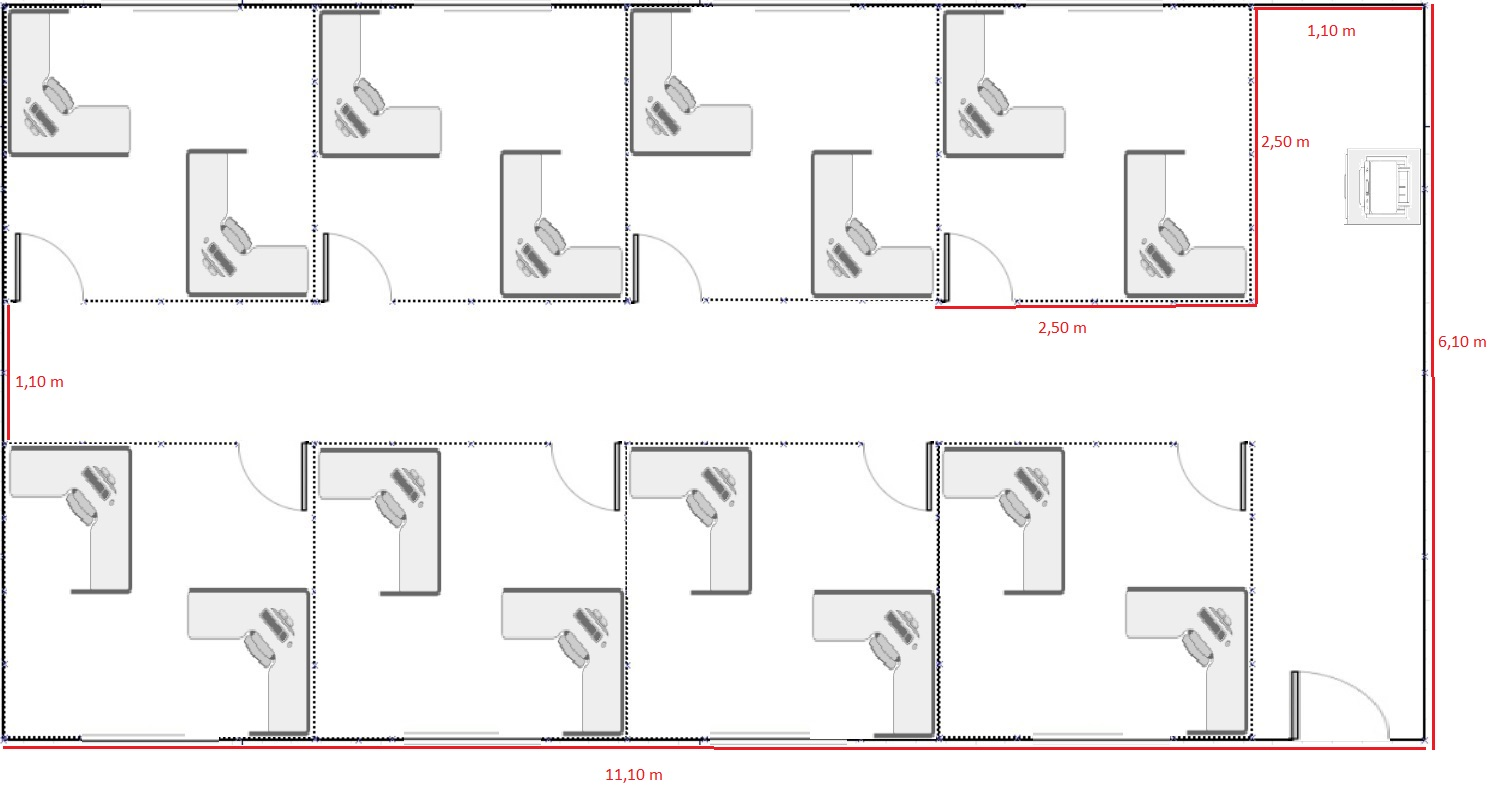
\includegraphics{fisica.jpg}
	\caption{Planta Física do Bloco E7}
	\label{fisica}
\end{figure}

\section{Planta Lógica - Elementos estruturados}

A figura \ref{logica} apresenta a planta lógica a ser implantada no projeto:

\begin{figure}
	\centering
	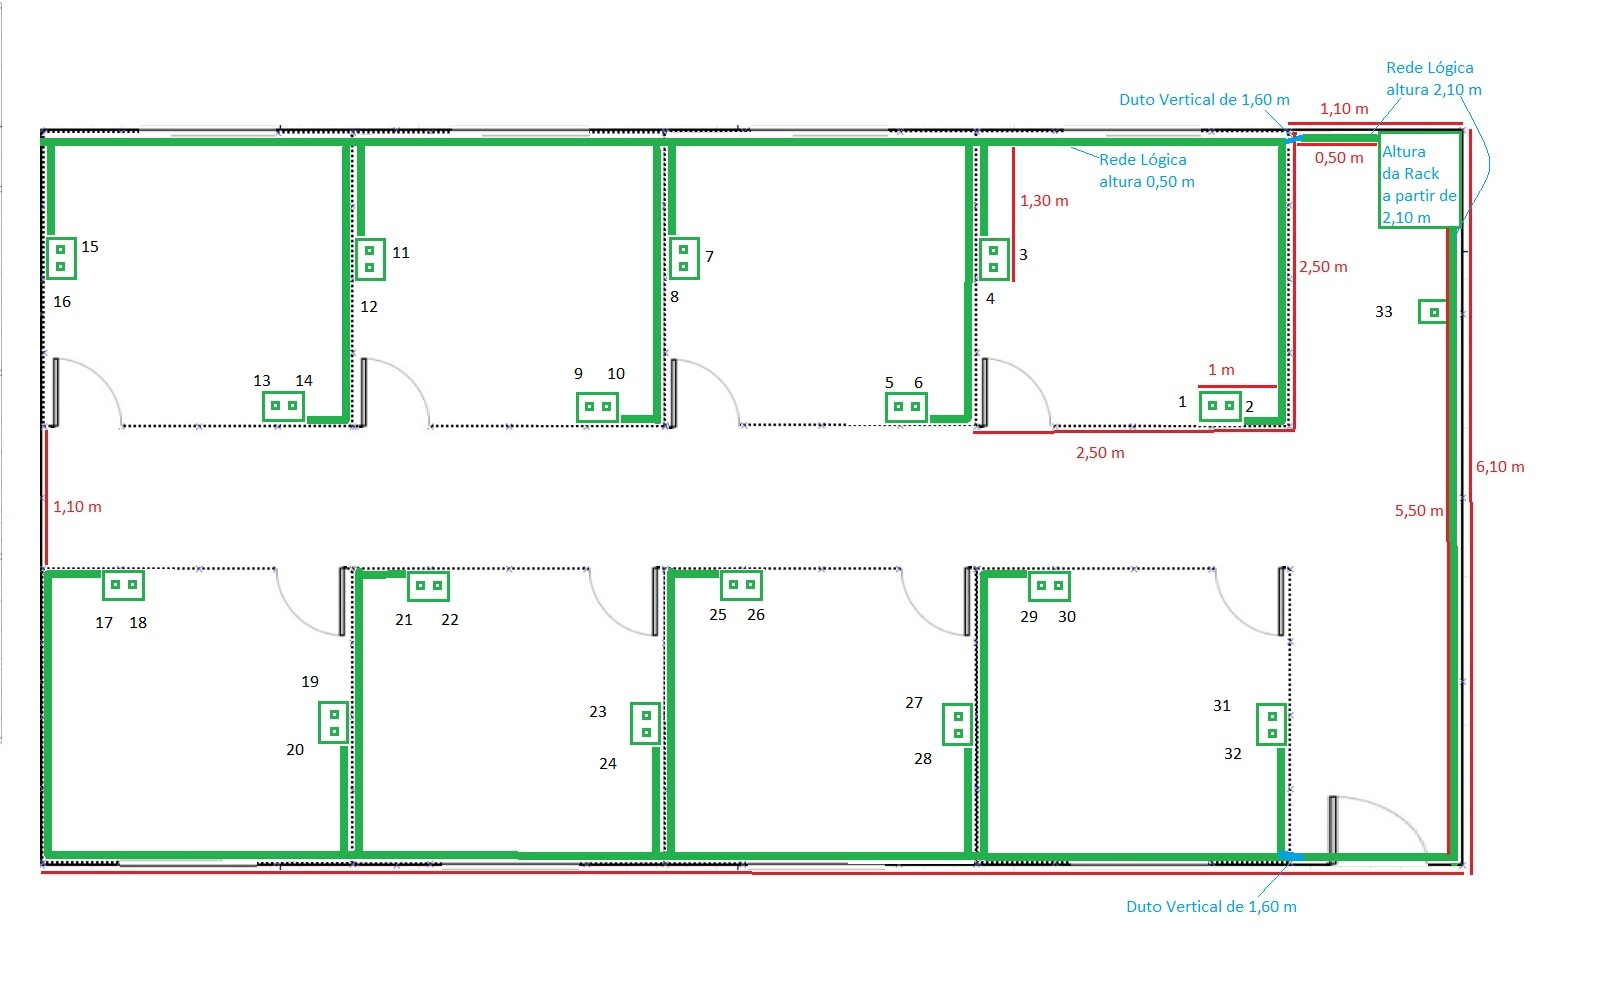
\includegraphics[]{logica.jpg}
	\caption{Planta Lógica do Bloco E7}
	\label{logica}
\end{figure}

\subsection{Estado atual}
Sem rede lógica. Somente conexão sem fio providas por Access Point e como receptor adaptadores wireless usb ou pci-express.

\subsection{Topologia}

A figura \ref{topologia} apresenta a Topologia a ser implantada no projeto:

\begin{figure}
	\centering
	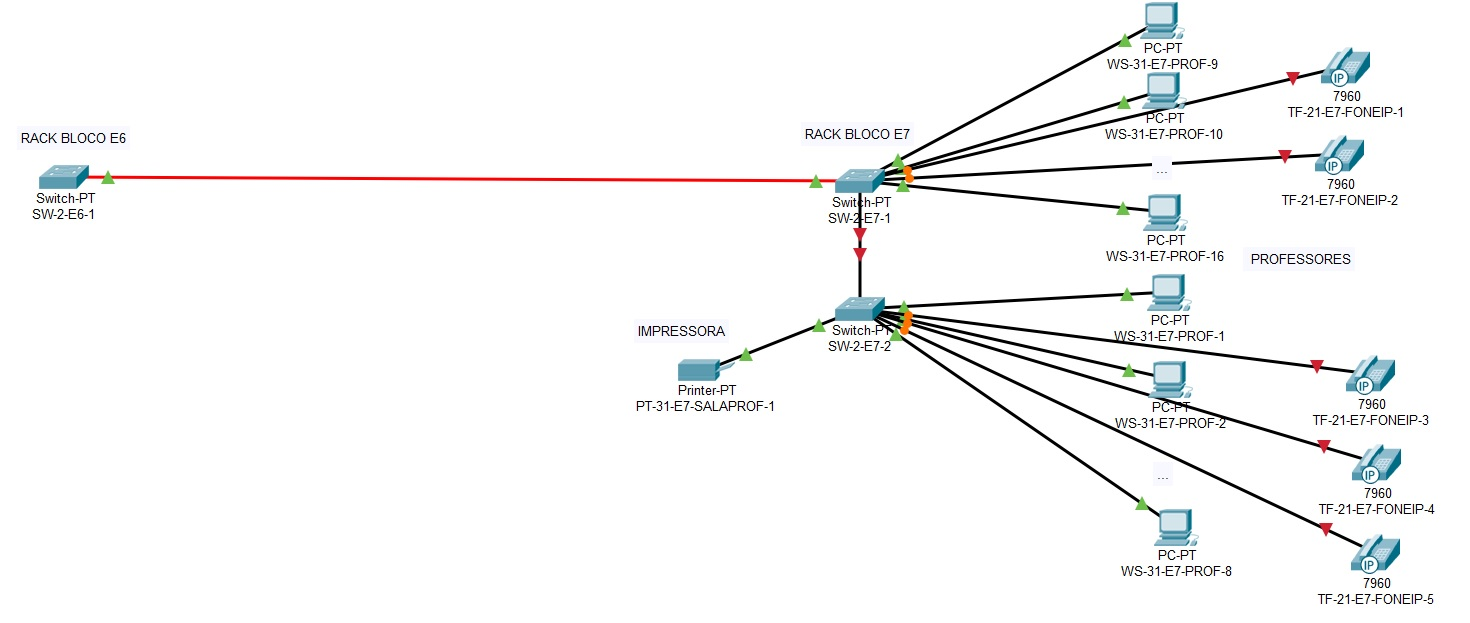
\includegraphics[]{topologia.jpg}
	\caption{Topologia do Bloco E7}
	\label{topologia}
\end{figure}

\subsection{Encaminhamento}

Material em que os cabos serão alojados/alocados:

Eletrodutos metálicos em formato U, totalizando 75 metros.


\subsection{Memorial descritivo}

Equipamentos passivos que serão utilizados:

\begin{table}[]
	\begin{tabular}{llll}
		EQUIPAMENTOS       		 & TIPO    & FABRICANTE & QUANTIDADE \\
		Rack              	 	 & 12U     & Furukawa   & 1 un       \\
		Switch           	  	 & SG-2860 & Cisco      & 2 un       \\
		Patch Panel       		 & 24P     & Furukawa   & 2 un       \\
		Cabo UTP           		 & CAT 6   & Furukawa   & 480 m      \\
		Ponteiras RJ-45 Fêmea    & CAT 6   & Furukawa   & 33 un      \\
		Patch Cords 1,5m  		 & CAT 6   & Furukawa   & 66 un     
	\end{tabular}
\end{table}

\subsection{Identificação dos cabos}

A identificação dos cabos seguirá padrão já adotado no restante do campus. Sendo assim, cada ponto recebe a letra do bloco e numeração sequencial conforme os pontos do patch panel.

Ponto 1 = E7-P01
Ponto 2 = E7-P02
Ponto...
Ponto 33 = E7-P33

\section{Implantação}
Cronograma de implantação - Atividade x tempo aproximado de execução.

ETAPA 01:
1 - Fixação da rack = 2 horas.
2 - Instalação das eletrocalhas nos pontos determinados no projeto = 1 semana.
3 - Passagem do cabeamento de lógica, inclusive o cabo provindo da estrutura de rede já existente = 1 semana.
ETAPA 02:
4 - Configuração e instalação de switchs e patch panels na rack = 4 horas.
5 - Crimpagem dos cabos nas extremidades dos patch panels e conectores RJ-45 fêmea nos pontos de acesso = 1 semana.
6 - Certificação dos pontos de lógica = 1 dia.
7 - Conectorização entre os switchs e patch panels = 1 hora.
ETAPA 03:
8 - Cabeamento dos equipamentos = 1 hora.
9 - Cadastro dos MAC dos equipamentos para atribuição de ip na rede cabeada = 1 hora.
10 - Remoção dos adaptadores wifi usb = 30 minutos.

Os itens 1, 2 e 3 serão executados pelo Departamento de Serviços Gerais com a utilização da equipe dos terceirizados já existentes no campus.
Todos os demais itens serão executados pela equipe da Coordenadoria de Gestão de Tecnologia de Informação do campus.

\section{Plano de certificação}
As etapas para a certificação serão:
Definição de data e horário; Definição da nomenclatura dos testes; Calibramento do equipamento; Testes dos cabos e Geração dos relatórios.

Para a certificação utilizar-se-a um certificador de rede Lantek6r. Os teste a serem realizados são:
Falha em wiremap,
wire length, resistance test, NEXT/FEXT, atenuação, perda de retorno, impedância, capacitância e falhas nos testes ACR e power sum ACR.

A certificação se dará nos Blocos E6 e E7. Os 33 novos pontos de lógica do Bloco E7 serão certificados, juntamente com a conexão de rede advinda do bloco E6.

Serão gerados relatórios de todos os testes citados.


\section{Plano de manutenção}

O plano de manutenção seguirá o já existente pois este projeto só agregará mais um ambiente cabeado aos demais já disponíveis e sob responsabilidade de manutenção da Cogeti no que tange aos equipamentos e ao Deseg com relação as eletrocalhas usadas para alojar o cabeamento.

\subsection{Plano de expansão}

Não há estimativa de crescimento nestes ambientes, pois o projeto já abrange o uso máximo dos espaços. Caso necessário novos pontos de lógica, ficarão disponíveis como sobra algumas portas dos equipamentos para tal, necessitando somente a passagem de novos cabos. As eletrocalhas para lógica também disponibilizará espaço extra para manobras.

\section{Risco}

Não detectamos riscos específicos ou significantes neste projeto. Somente queda dos equipamentos no manuseio ou configuração inadequada dos equipamentos podendo influenciar negativamente na rede.

\begin{table}[]
	\begin{tabular}{llll}
		EQUIPAMENTO                 & QUANTIDADE  & CUSTO UNITÁRIO        & CUSTO TOTAL   \\
		Rack 12 U                   & 1 un        & R\$ 550,00            & R\$ 550,00    \\
		Switch Cisco SG-2960        & 2 un        & R\$ 2.249,00          & R\$ 4.498,00  \\
		Patch Panel                 & 2 un        & R\$ 240,00            & R\$ 480,00    \\
		Eletrocalhas                & 25 un x 3 m & R\$ 28,90             & R\$ 722,50    \\
		Cabo UTP CAT 6              & 480 m       & R\$ 598,00 (cx 305 m) & R\$ 940,00    \\
		Ponteiras RJ-45 Fêmea CAT 6 & 33 un       & R\$ 15,10             & R\$ 498,30    \\
		Patch Cords 1,5 m CAT 6     & 66 un       & R\$ 39,90             & R\$ 2.633,40  \\
		\multicolumn{3}{l}{TOTAL}                                         & R\$ 10.322,20
	\end{tabular}
\end{table}

\section{Referências bibliográficas}
%Utilize o mendley, o jabref ou diretamente o bibtex para gerenciar suas referências biliográficas. As referências são criadas automaticamente de acordo com o uso no texto.

%Exemplo: Redes de computadores, segundo \cite{t2013} é considerada..... Já \cite{kurose2010} apresenta uma versão...

%Analisando os pressupostos de \cite{ref3} e \cite{ref4} concluimos que....

\renewcommand\refname{} %%Referências bibliográficas}  
\bibliographystyle{ieeetr}
\bibliography{referencias}  

\end{document}